\documentclass[12pt]{article}

\title{Symbolic Logic HW 5}
\author{Tyler Tracy}

\usepackage{amsmath}
\usepackage{amssymb}
\usepackage{graphicx}
\graphicspath{ {./imgs/} }

\begin{document}

\section*{Problem 1}

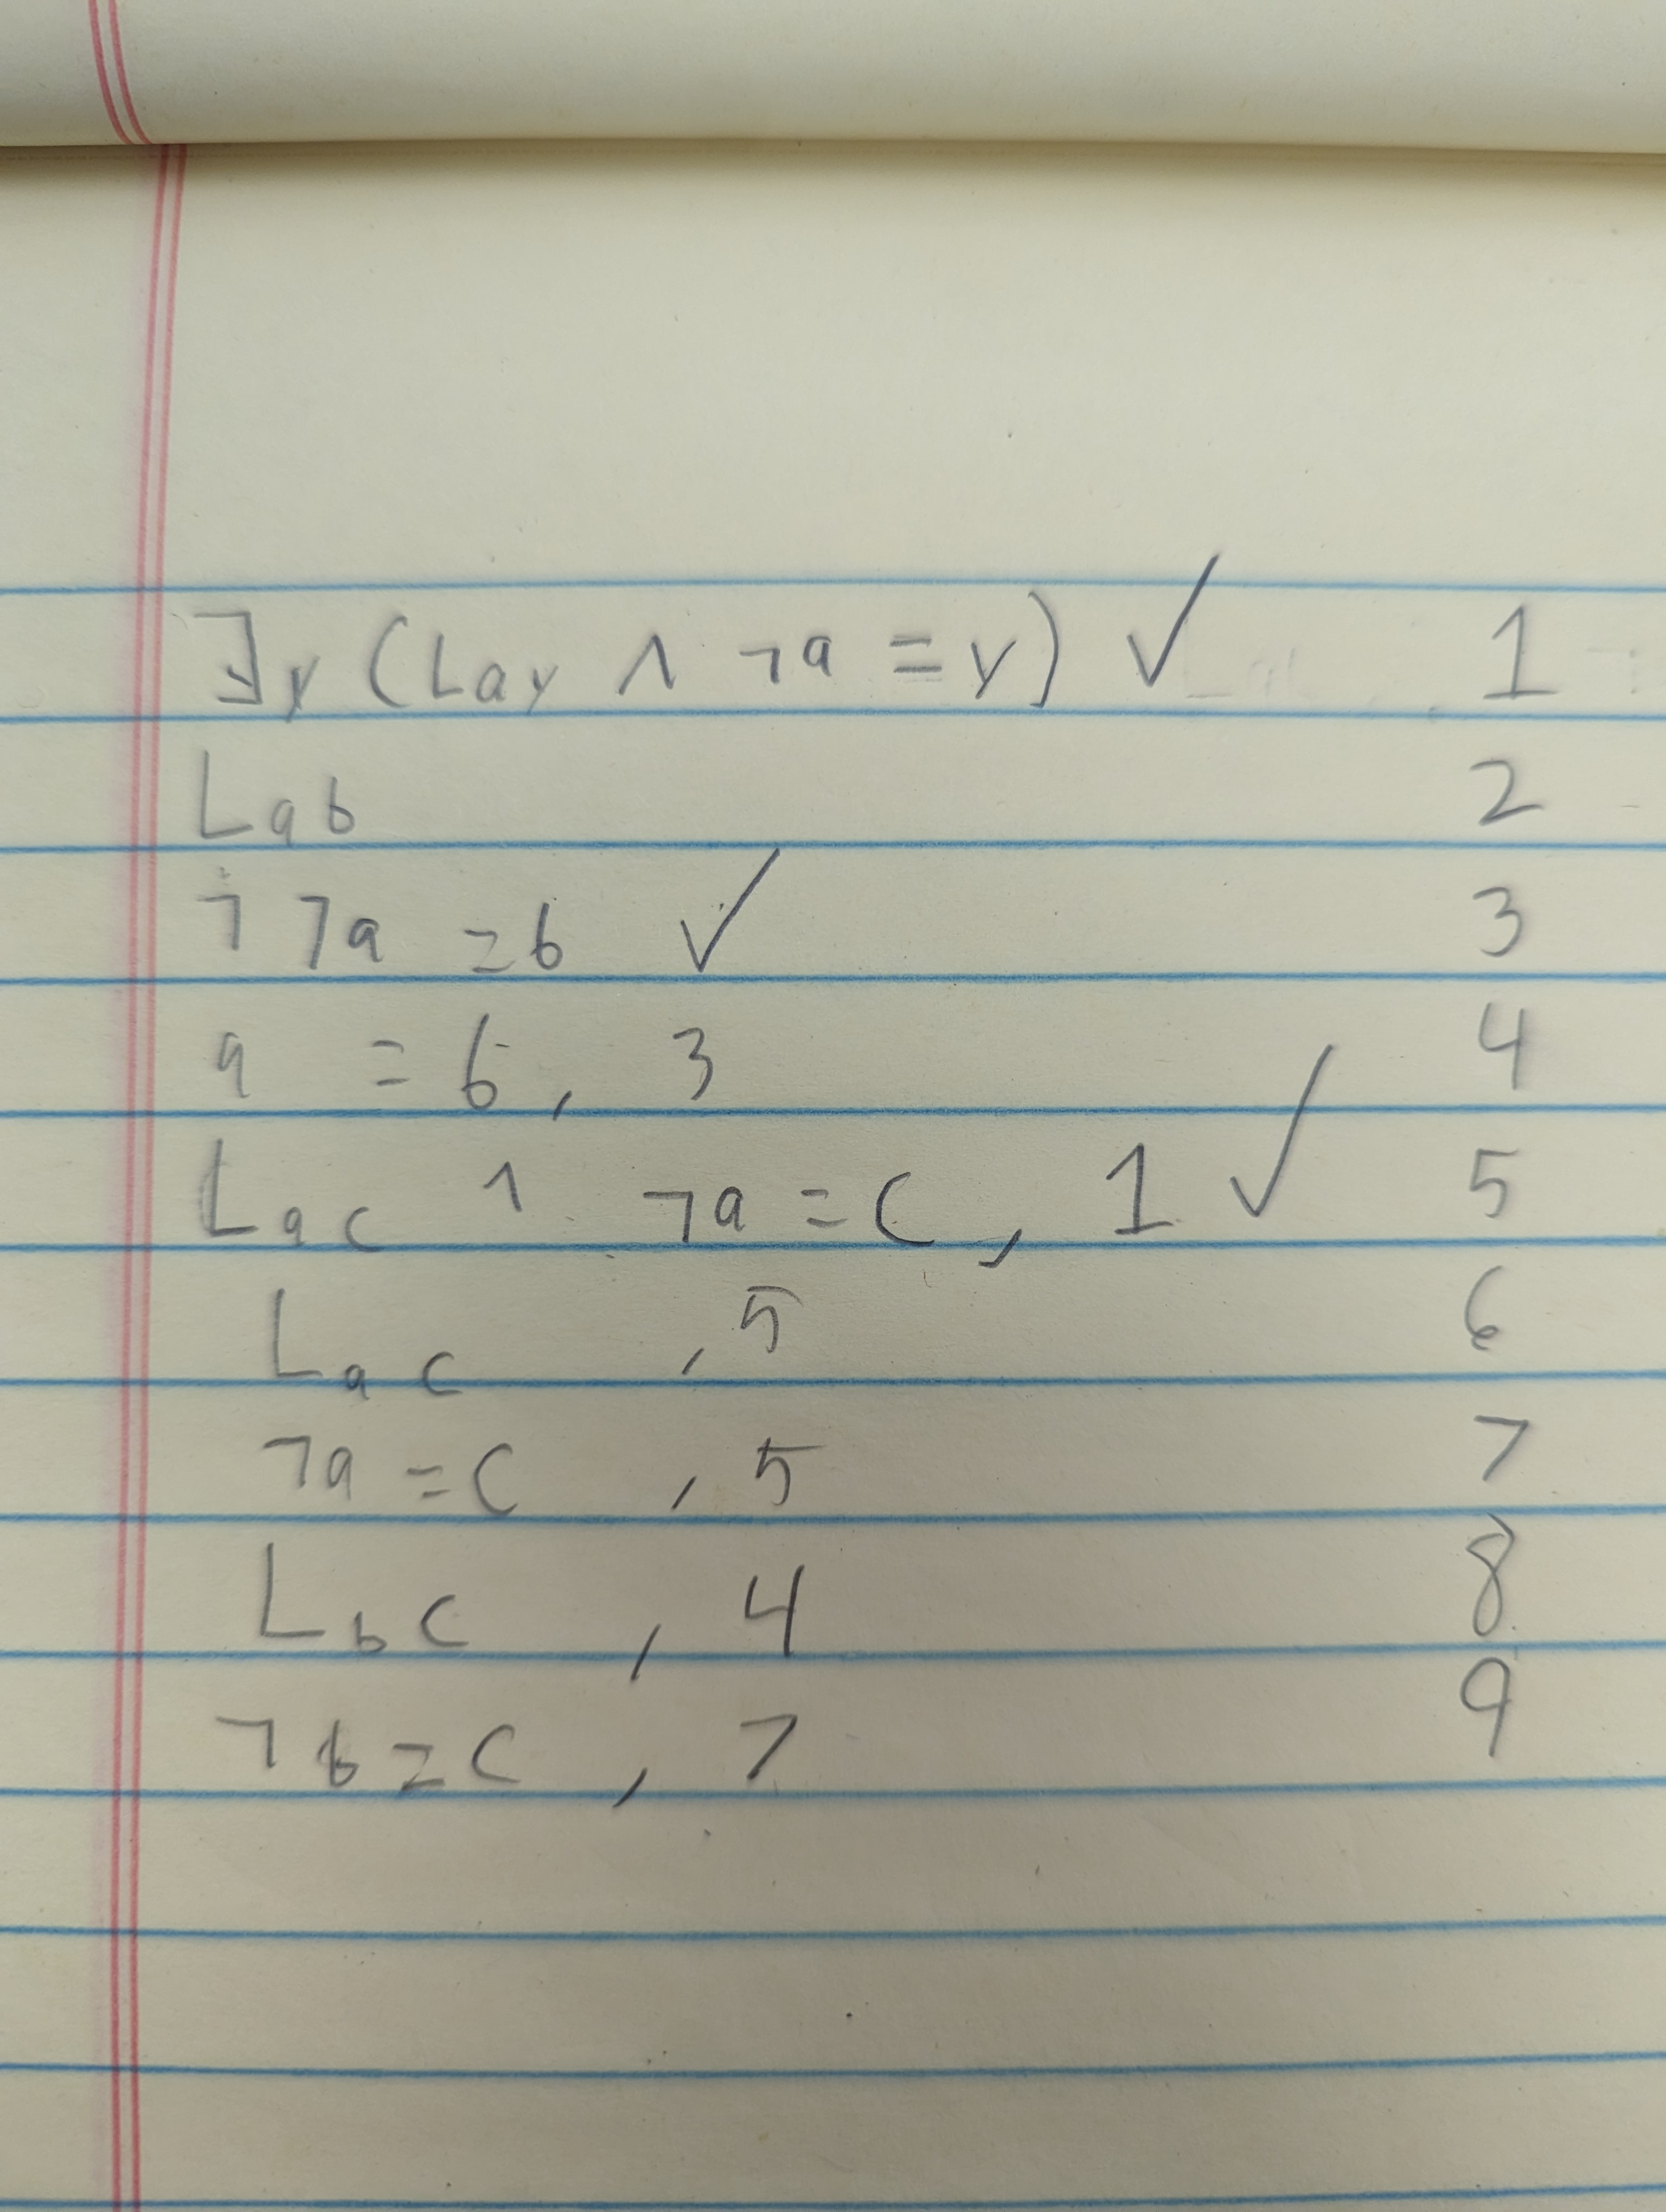
\includegraphics[width=\textwidth]{1}

This argument is invalid. Here is an interpretation that makes it false. 

Domain $ = \{1, 2\}$

$a \rightarrow 1$

$b \rightarrow 1$

$c \rightarrow 2$

$L \rightarrow {<1, 1>, <1, 2>}$


$\exists y (Lay \land a \lnot = y)$ (This is true $y = c$)

$Lab$ (This is true L contains $<1, 1>$)

$a \lnot = b$ (This is false $a = b = 1$)

The premises are true, but the conclusion is false. This is an invalid argument


\section*{Problem 2}

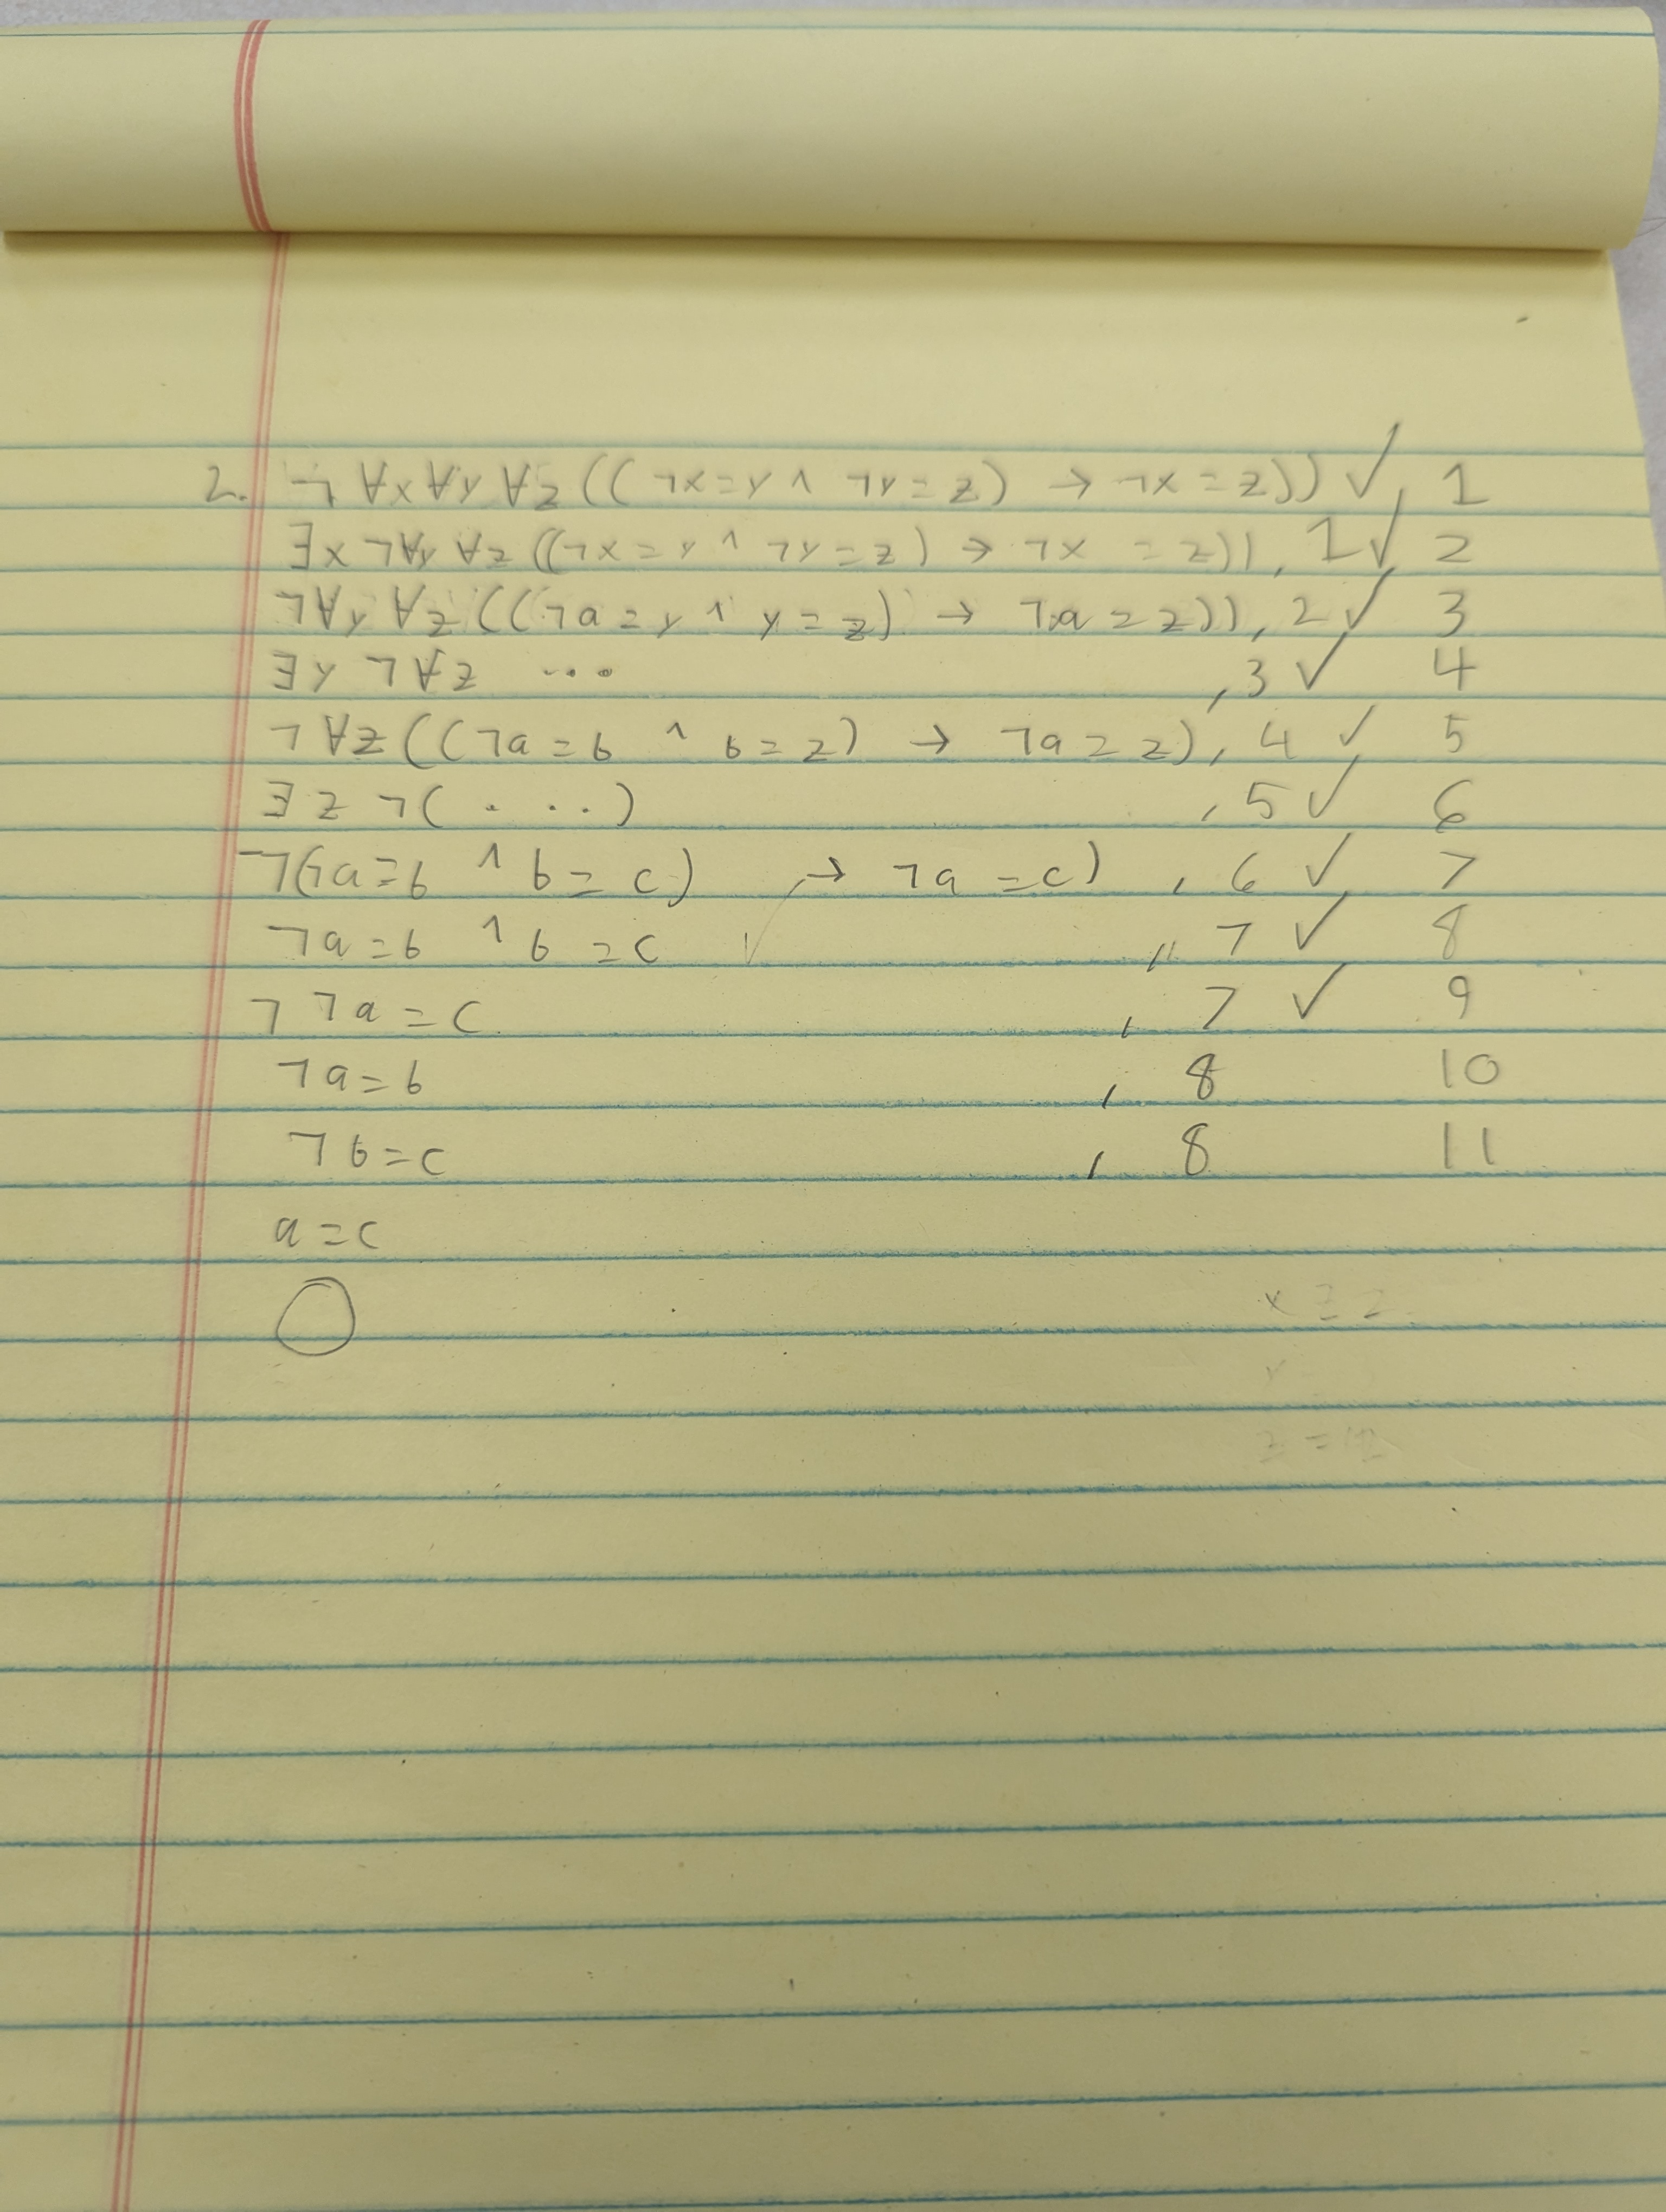
\includegraphics[width=\textwidth]{2}

This statement is not a logical truth. Here is an interpretation that makes it false. 

Domain $ = \{1, 2\}$

$a \rightarrow 1$

$b \rightarrow 2$

$c \rightarrow 3$

It is not true that the inner predicate holds over the entire domain. If $x = a, y= b, z = c$ then $x \lnot = y$ and $y \lnot = z$ but $x = z$. So this is false. 


\section*{Problem 3}

\subsection*{Part A}

The black cat is on the mat. 

$\exists (Bx \land Cx \land Mx \land forall y (Cy \land By \rightarrow y = x))$

So some cat is on the mat is black.

$\exists x (Cx \land Mx \land Bx)$

This is valid, here is the tree

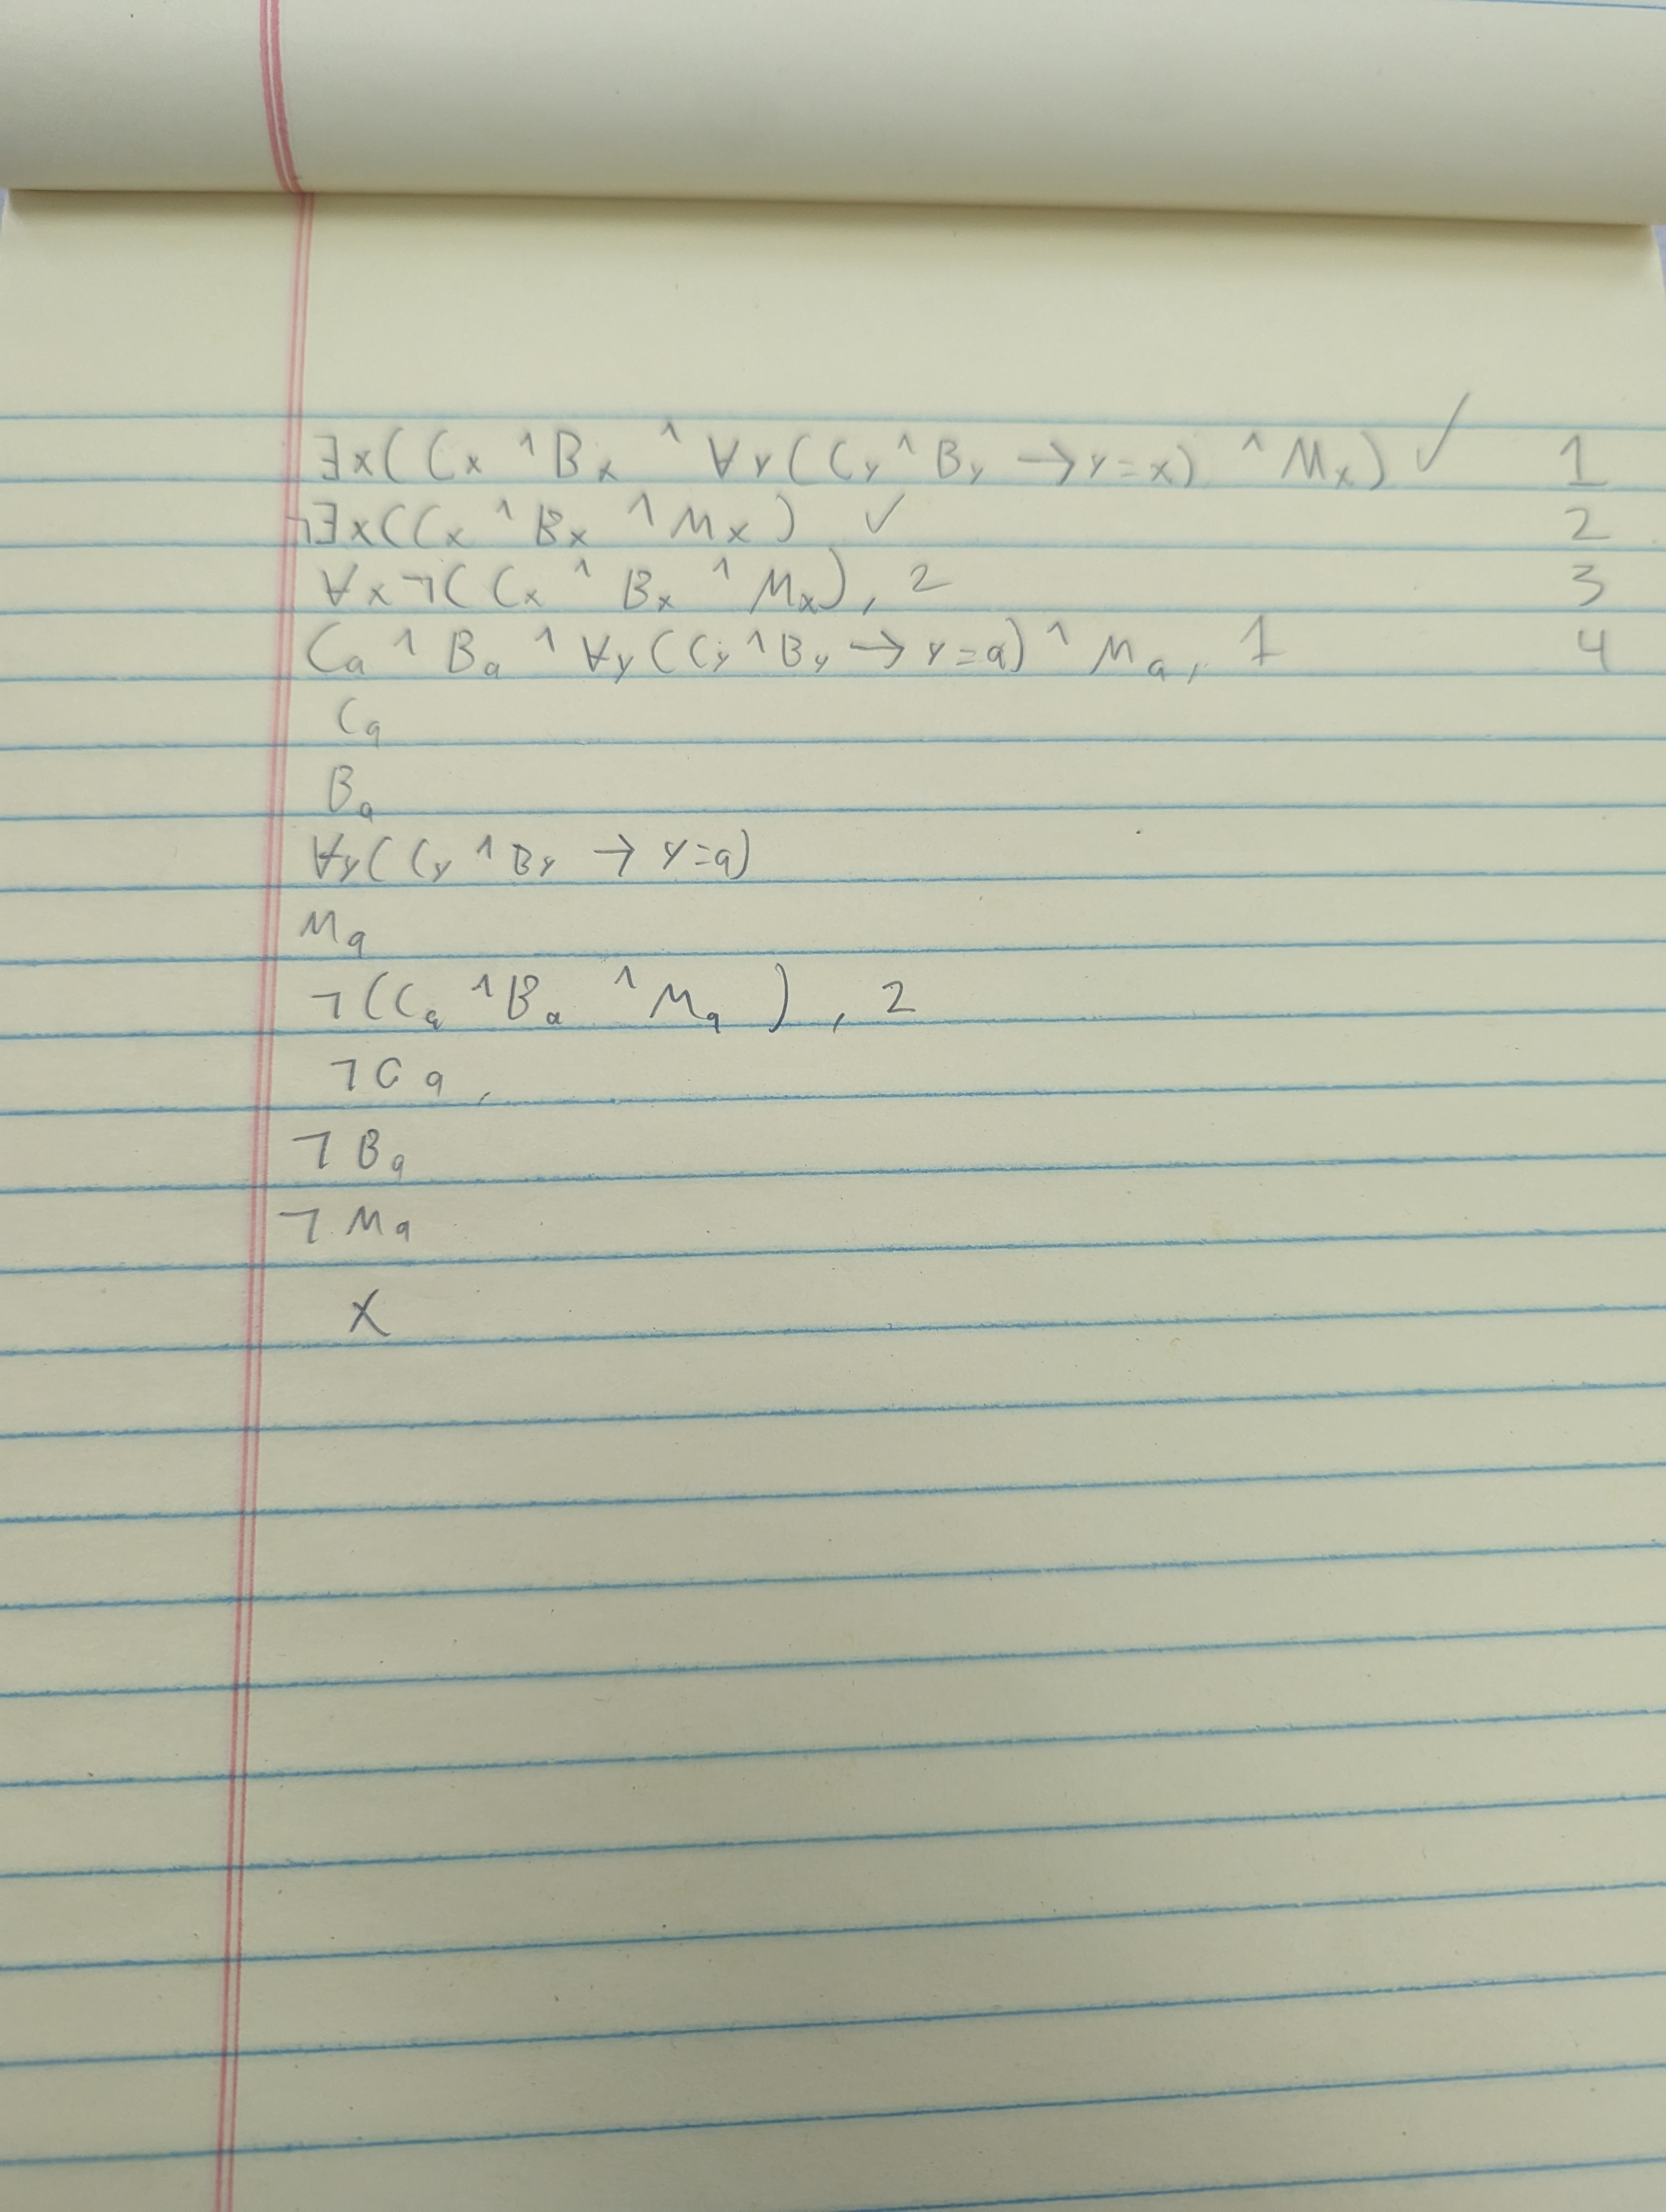
\includegraphics[width=\textwidth]{3a}

\subsection*{Part B}

The gray cat is on the mat. 

$\exists (Gx \land Cx \land Mx \land forall y (Cy \land Gy \rightarrow y = x))$

So, every cat is on the mat

$\forall x (Cx \land Mx \rightarrow Gx)$

This is invlaid, he is an interpretation that makes it false. 

Domain = $\{FuzzyCat, TabbyCat\}$

$M = {FuzzyCat}$
$G = {FuzzyCat}$
$C = {FuzzyCat, TabbyCat}$

So the FuzzyCat is on the mat, but it is not the case that all cats are on the mat because the TabbyCat is a cat but not on the mat. 

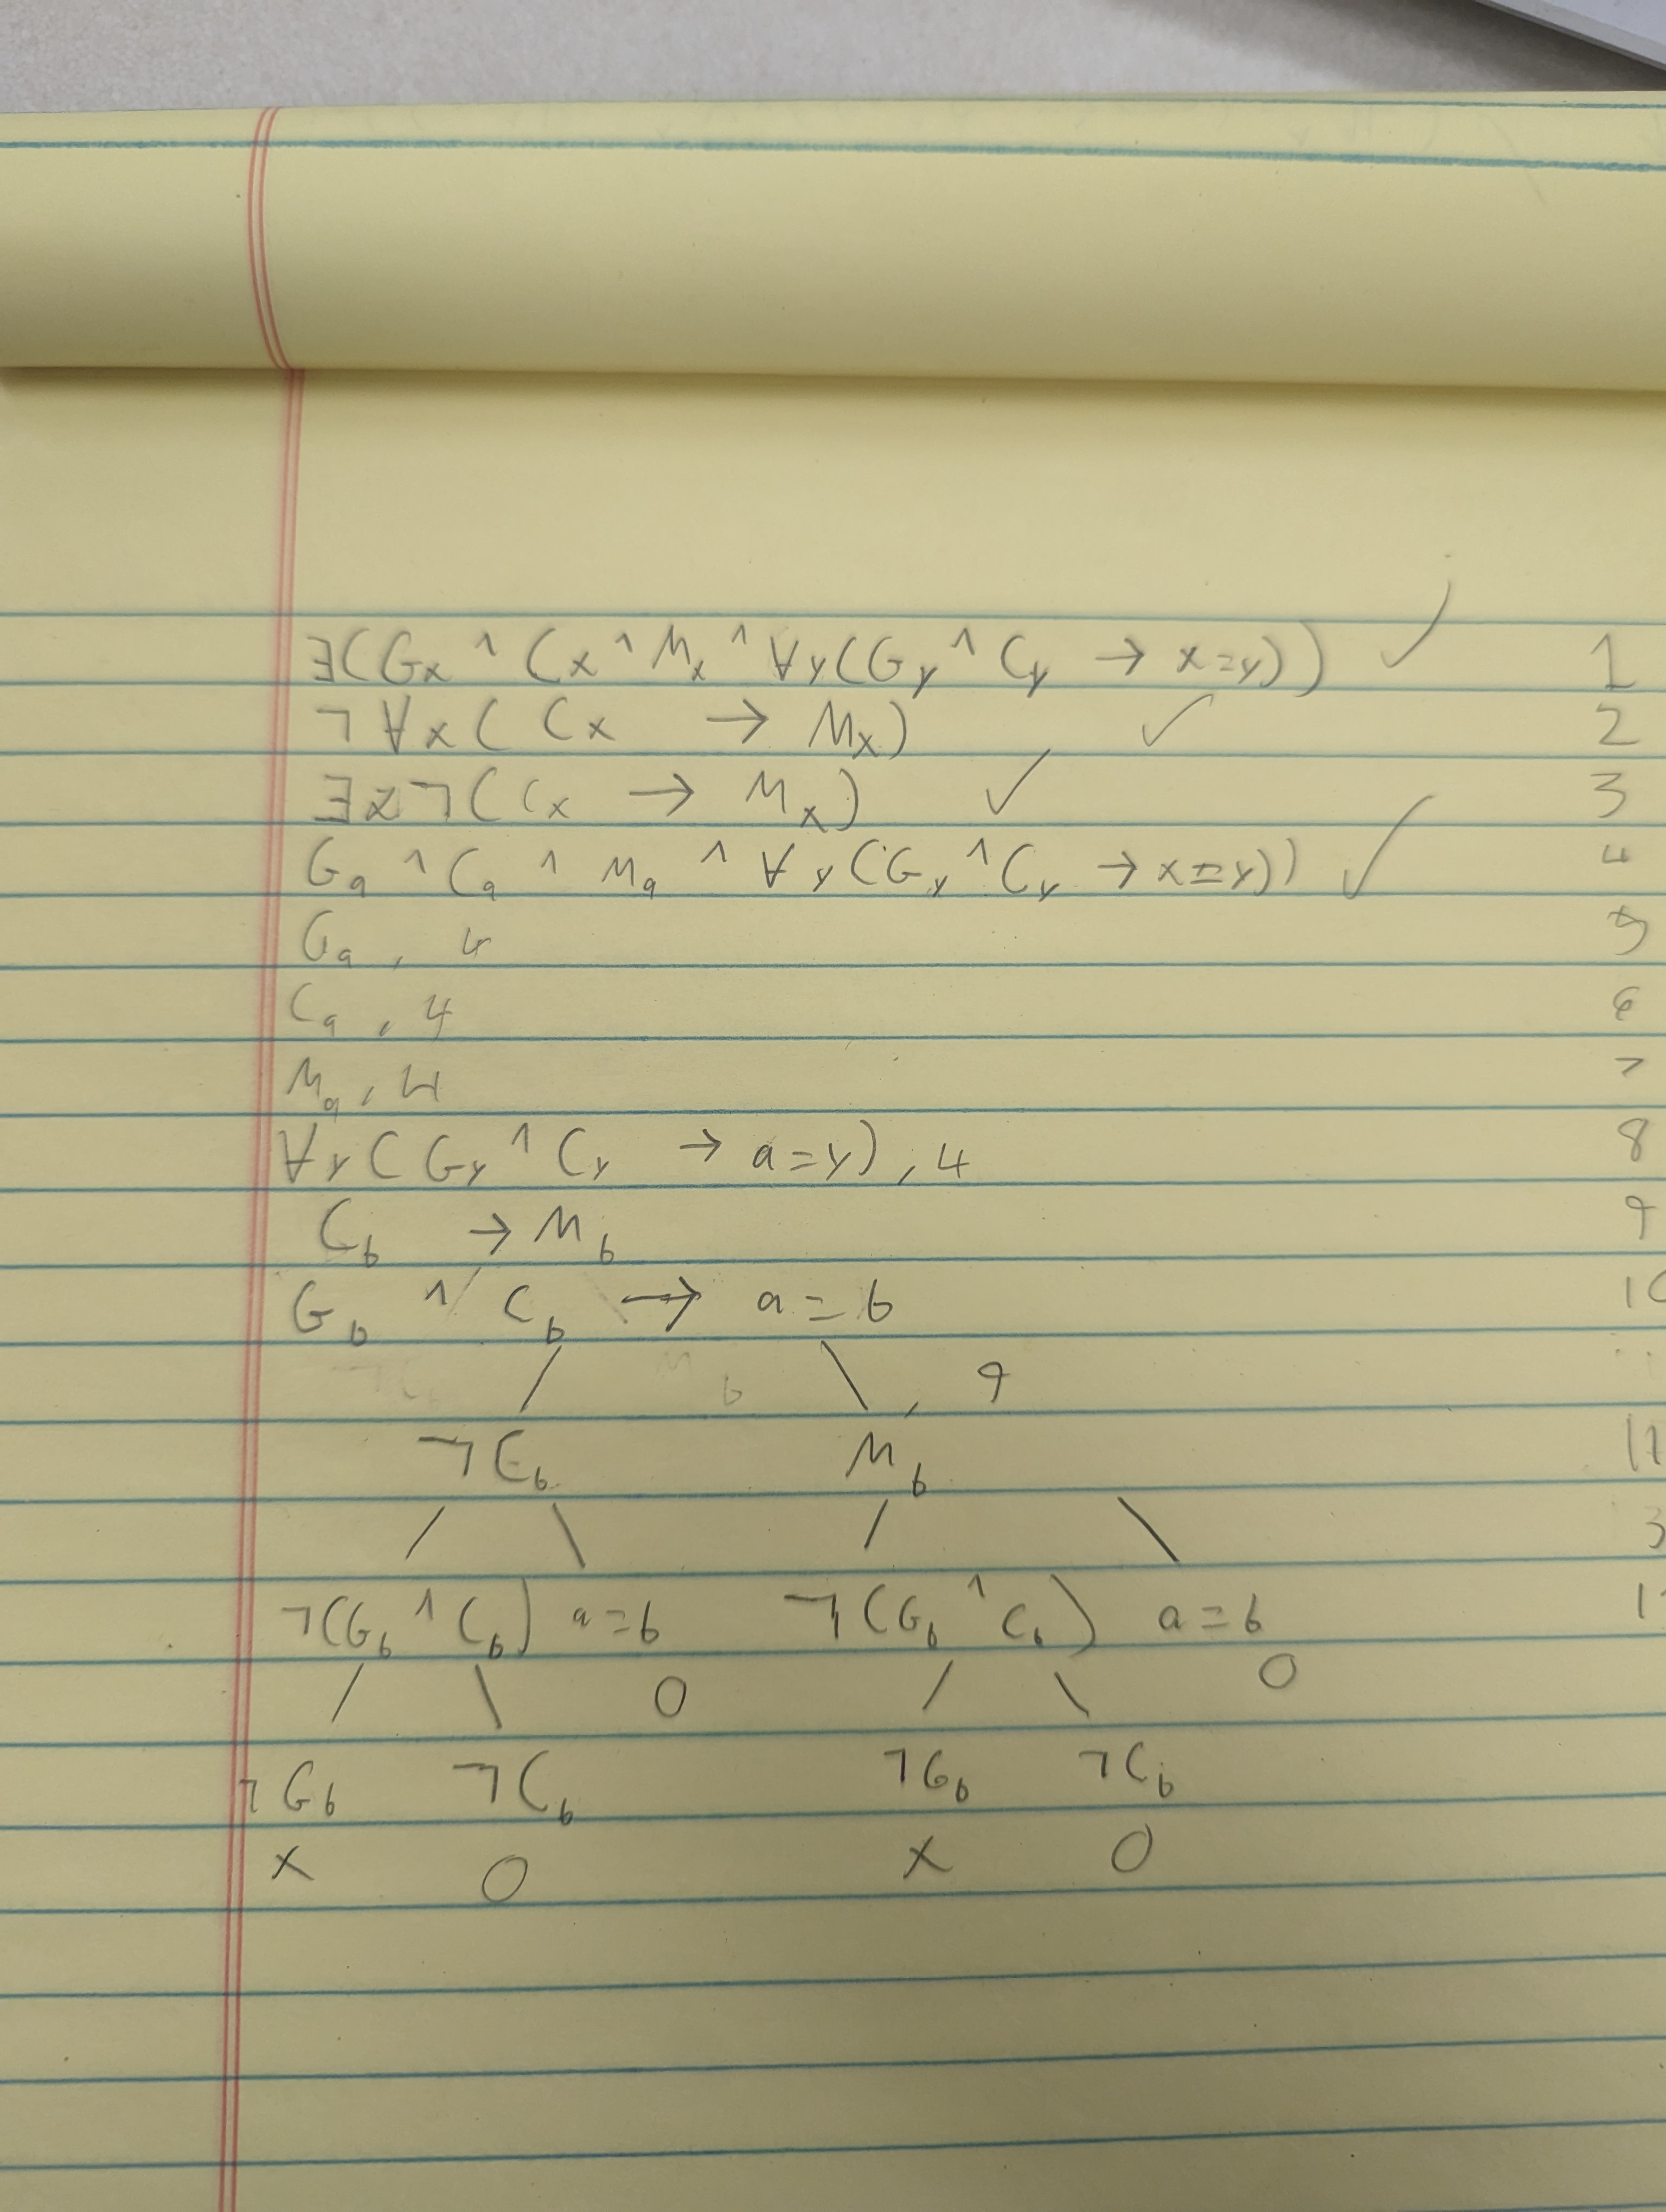
\includegraphics[width=\textwidth]{3b}


\section*{Problem 4}

(a) Everyone likes at least one person. 

$\forall x \exists y Lxy$

(b) Everyone likes at most one person. 

$\forall x \forall y \forall z ((Lxy \land Lxz) \rightarrow y = z)$

(c) Everyone likes exactly one person. 

$\forall x (\exists y Lxy \land \forall z (Lxz \rightarrow y = z))$

(d) Everyone likes at least two people. 

$\forall x \exists y \exists z Lxy \land Lxz \land y \lnot = z$

(e) Everyone likes at most two people. 

$\forall x \forall y \forall z \forall w ((Lxy \land Lxz \land Lyz) \rightarrow (w = x \lor w = y \lor w = z))$

(f) Everyone likes exactly two people. 

$\forall x \exists y \exists z Lxy \land Lxz \land \forall w ((Lxw \land y \lnot = w \land z \lnot = w) \rightarrow y = z)$

(g) Everyone like only themselves [i.e. we like ourselves and no-one else] 

$\forall x \forall y (Lxx \land (Lxy \rightarrow x = y))$

(h) Everyone likes some other person [i.e. someone other than themself] 

$\forall x \exists y (Lxy \land x \lnot = y)$

(i) Some people like only other people [i.e. people other than themself] 

$\exists x \forall y (Lxy \land x \lnot = y)$

(j) Only Art likes Betty. 

$\forall x (Lxb \rightarrow x = a)$

(k) The tall person likes Art 

$\exists x (Tx \land Lxa \land \forall y ( Ty \rightarrow x = y) )$

(l) The person who likes Art likes Betty 

$\exists x (Lxa \land \forall y (Lya \rightarrow y = x) \land Lxb)$

(m) The person whom Art likes likes Betty. 

$\exists x (Lax \land \forall y (Lay \rightarrow y = x) \land Lxb)$

(n) Betty likes the person whom Art likes 

$\exists x (Lbx \land \forall y (Lay \rightarrow y = x) \land Lax)$

(o) Art likes tall people 

$\forall x (Tx \rightarrow Lax)$

\section*{Problem 5}

$\exists x (x = fj \land x = mj) \rightarrow \exists x Pxj$

If someone is the father or mother of jack, then they are the parent of jack. 

$\lnot \exits x Pjx \rightarrow \exits x Gjx$

If jack isn't a parent, then jack isn't a grandparent. 

$\exists xGffjx$

Jack's father's father is a grandparent to someone.  

$\exists x([(Pxj \land \lnot x = mj) \land \forall y((Pyj \land \lnot y = mj) \rightarrow x = y)] \land x = fj) $

Jack's parent who is not his mother is his father. 

Laura is Jack’s mother 

$l = mj$

Laura is a parent of Jack. 

$Plj$

The father of Jack’s mother is a grandparent of Jack. 

$Gfmjj$

If Laura is Jack’s mother, then Jack is Laura’s son 

$l = mj \rightarrow j = sl$

Jack’s mother’s mother is not a parent of Jack. 

$\lnot Pmmjj$ 

(j) If Jack has a father, then Jack has a parent

$\exists x x = fj \rightarrow \exists x Pxj$

\end{document}
